\begin{frame}[fragile]
  \frametitle{Norms \& distance measures in R}
  %% \framesubtitle{}

\ungap
\begin{alltt}\small
\REM{We will use the cooccurrence matrix \textbf{M} from the last session}
> print(M)  \begin{Rout}
        eat get hear kill see use
  boat    0  59    4    0  39  23
  cat     6  52    4   26  58   4
  cup     1  98    2    0  14   6
  dog    33 115   42   17  83  10
  knife   3  51    0    0  20  84
  pig     9  12    2   27  17   3
\end{Rout}
\REM{Note: you can save selected variables with the \texttt{save()} command,}
\REM{and restore them in your next session (similar to saving R's workspace)}
> save(M, O, E, M.mds, file="dsm_lab.RData")

\REM{\texttt{load()} restores the variables under the same names!}
> load("dsm_lab.RData")
\end{alltt}
\end{frame}

\begin{frame}[fragile]
  \frametitle{Norms \& distance measures in R}
  %% \framesubtitle{}

\ungap
\begin{alltt}\small    
\REM{Define functions for general Minkowski norm and distance;}
\REM{parameter \emph{p} is optional and defaults to \emph{p} = 2}
> p.norm <- function (x, p=2) (sum(abs(x)^p))^(1/p)
> p.dist <- function (x, y, p=2) p.norm(x - y, p)

> round(apply(M, 1, p.norm, p=1), 2) \begin{Rout}
 boat   cat   cup   dog knife   pig 
  125   150   121   300   158    70 \end{Rout}
> round(apply(M, 1, p.norm, p=2), 2) \begin{Rout}
  boat    cat    cup    dog  knife    pig 
 74.48  82.53  99.20 152.83 100.33  35.44 \end{Rout}
> round(apply(M, 1, p.norm, p=4), 2) \begin{Rout}
  boat    cat    cup    dog  knife    pig 
 61.93  66.10  98.01 122.71  86.78  28.31 \end{Rout} 
> round(apply(M, 1, p.norm, p=99), 2) \begin{Rout}
 boat   cat   cup   dog knife   pig 
   59    58    98   115    84    27  \end{Rout}
\end{alltt}
\end{frame}

\begin{frame}[fragile]
  \frametitle{Norms \& distance measures in R}
  %% \framesubtitle{}

\ungap
\begin{alltt}\small    
\REM{Here's a nice trick to normalise the row vectors quickly}
> normalise <- function (M, p=2) M / apply(M, 1, p.norm, p=p)

\REM{\texttt{dist()} function also supports Minkowski \emph{p}-metric}
\REM{(must normalise rows in order to compare different metrics)}
> round(dist(normalise(M, p=1), method="minkowski", p=1), 2) \begin{Rout}
      boat  cat  cup  dog knife
cat   0.58                     
cup   0.69 0.97                
dog   0.55 0.45 0.89           
knife 0.73 1.01 1.01 1.00      
pig   1.03 0.64 1.29 0.71  1.28 \end{Rout}

\REM{Try different \emph{p}-norms: how do the distances change?}
> round(dist(normalise(M, p=2), method="minkowski", p=2), 2)
> round(dist(normalise(M, p=4), method="minkowski", p=4), 2)
> round(dist(normalise(M, p=99), method="minkowski", p=99), 2)
\end{alltt}
\end{frame}

\begin{frame}[c]
  \frametitle{Why it is important to normalise vectors}
  \framesubtitle{before computing a distance matrix}

  \begin{center}
    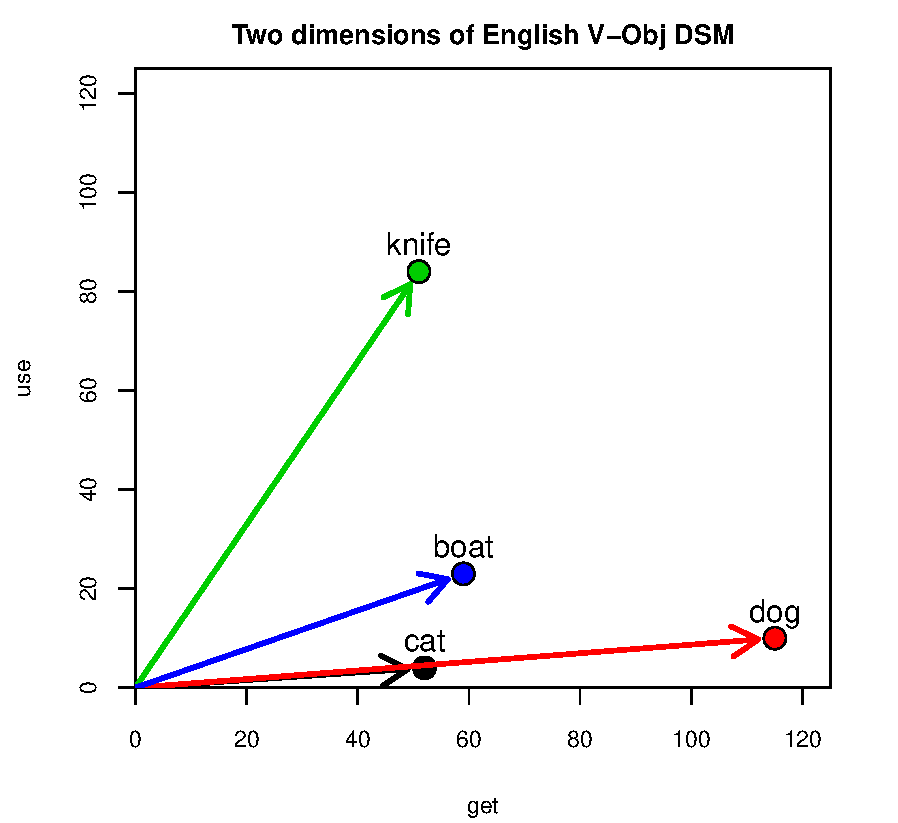
\includegraphics[width=7cm]{img/hieroglyph_2d_3}
  \end{center}
\end{frame}

%%% Local Variables: 
%%% mode: latex
%%% TeX-master: "../../workspace"
%%% End: 
